\chapter{Другие виды модификации данных}
\section{Использование
объекта последовательности
и свойства столбца IDENTITY}



При вставке строки в таблицу не нужно указывать значение для столбца IDENTITY,
поскольку он получает свое значение автоматически.

В случаях, когда при вставке строк в таблицу вы хотите указать собственные значения для столбца orderid, необходимо установить параметр сеанса, который называется SET IDENTITY\_INSERT <table> to ON.

В языке T-SQL имеется несколько функций, которые можно использовать, чтобы
запросить последнее сгенерированное значение идентификатора, например, если
оно вам необходимо, когда вы выполняете вставку связанных строк в другую таблицу:

\begin{itemize}
	\item функция SCOPE\_IDENTITY возвращает последнее значение идентификатора, сгенерированное в вашем сеансе в данной области; 
	\item функция @@IDENTITY возвращает последнее значение идентификатора, сгенерированное в вашем сеансе независимо от области; 
	\item функция IDENT\_CURRENT принимает в качестве входа таблицу и возвращает последнее значение идентификатора, сгенерированное во входной таблице независимо от сессии. 
\end{itemize}

\begin{lstlisting}[label=lst:funcReturn, language=sql]
	SELECT
	SCOPE_IDENTITY() AS SCOPE_IDENTITY,
	@@IDENTITY AS [@@IDENTITY],
	IDENT_CURRENT('Sales.MyOrders') AS IDENT_CURRENT; 
\end{lstlisting}

\subsection{Использование объекта последовательности}

В отличие от свойства
столбца IDENTITY, последовательность — это независимый объект базы данных.
Объект последовательности лишен многих ограничений, присущих свойству
IDENTITY, к которым относятся следующие. 

\begin{itemize}
	\item Свойство IDENTITY привязано к конкретному столбцу в определенной таблице.
	Вы не можете удалить свойство, уже существующее у столбца, а также добавить
	это свойство существующему столбцу. Столбец должен быть определен с этим
	свойством.
	\item Иногда нужно, чтобы ключи не конфликтовали в разных таблицах, но свойство
	IDENTITY определяется на уровне таблицы. 
	\item Иногда требуется сгенерировать значение до его использования. Это невозможно при использовании свойства IDENTITY. Необходимо вставить строку и только
	потом получить новое значение с помощью функции. 
	\item Нельзя обновить столбец IDENTITY. 
	\item Свойство IDENTITY не поддерживает циклическое повторение. 
	\item Инструкция TRUNCATE сбрасывает свойство идентификатора. 
\end{itemize}

Объект последовательности создается как независимый объект базы. Он не привязан к определенному столбцу в определенной таблице. Для создания последовательности можно использовать команду CREATE SEQUENCE. Как минимум, следует
указать имя объекта: 

\begin{lstlisting}[label=lst:funcReturn, language=sql]
	CREATE SEQUENCE <schema>.<object>;
\end{lstlisting}

Далее приведен пример для определения последовательности, которую можно использовать для генерации идентификаторов заказов. 

\begin{lstlisting}[label=lst:funcReturn, language=sql]
	CREATE SEQUENCE Sales.SeqOrderIDs AS INT
 		MINVALUE 1
 		CYCLE;
\end{lstlisting}


Чтобы запросить новое значение из последовательности, следует использовать
функцию NEXT VALUE FOR <sequence name>. Например, выполните следующий код
три раза:

\begin{lstlisting}[label=lst:funcReturn, language=sql]
	SELECT NEXT VALUE FOR Sales.SeqOrderIDs; 
\end{lstlisting}

Если вам необходимо изменить текущее значение, сделать это можно, используя следующий код: 
\begin{lstlisting}[label=lst:funcReturn, language=sql]
	ALTER SEQUENCE Sales.SeqOrderIDs RESTART WITH 1;  
\end{lstlisting}


Далее приведен пример использования функции NEXT VALUE FOR в предложении
INSERT VALUES, которое вставляет три строки в таблицу. 

\begin{lstlisting}[label=lst:funcReturn, language=sql]
	INSERT INTO Sales.MyOrders(orderid, custid, empid, orderdate) VALUES
	(NEXT VALUE FOR Sales.SeqOrderIDs, 1, 2, '20120620'),
	(NEXT VALUE FOR Sales.SeqOrderIDs, 1, 3, '20120620'),
	(NEXT VALUE FOR Sales.SeqOrderIDs, 2, 2, '20120620'); 
\end{lstlisting}


Также можно использовать функцию NEXT VALUE FOR в ограничении DEFAULT, что
позволяет ограничению автоматически генерировать значения в процессе вставки
строк. Чтобы определить такое ограничение DEFAULT для столбца orderid, выполните следующий код:

\begin{lstlisting}[label=lst:funcReturn, language=sql]
	ALTER TABLE Sales.MyOrders
	ADD CONSTRAINT DFT_MyOrders_orderid
	DEFAULT(NEXT VALUE FOR Sales.SeqOrderIDs) FOR orderid;
\end{lstlisting}

Существует очень большая разница в производительности между использованием
NO CACHE и CACHE <some value>.

Если установлен параметр NO CACHE, SQL Server должен делать запись на диск для каждого запроса нового значения последовательности. Но с кэшированием производительность намного выше. По умолчанию в момент написания этого курса значение кэша устанавливалось равным 50.

\begin{lstlisting}[label=lst:funcReturn, language=sql]
	ALTER SEQUENCE Sales.SeqOrderIDs
	CACHE 100; 
\end{lstlisting}

Возвращаясь к списку ограничений свойства IDENTITY, о которых говорилось ранее,
перечислим преимущества объекта последовательности. 

\begin{itemize}
	\item Объект последовательности не привязан к конкретному столбцу в определенной
	таблице. При желании можно указать новое значение с помощью ограничения
	DEFAULT. Это ограничение можно добавить к существующему столбцу или удалить у него. 
	\item Поскольку последовательность — это независимый объект базы данных, можно
	применять ту же последовательность для генерации ключей, которые используются в разных таблицах. Таким образом, не будет конфликта ключей в разных
	таблицах. 
	\item Можно сгенерировать значение последовательности до его использования, сохраняя результат функции NEXT VALUE FOR в переменной. 
	\item Можно обновлять столбцы с помощью инструкции UPDATE, используя результаты функции NEXT VALUE FOR. 
	\item Объект последовательности поддерживает циклическое повторение. 
	\item Инструкция TRUNCATE не сбрасывает текущее значение объекта последовательности, поскольку последовательность не зависит от использующих ее таблиц. 
\end{itemize}

\begin{figure}[h!]
	\begin{center}
		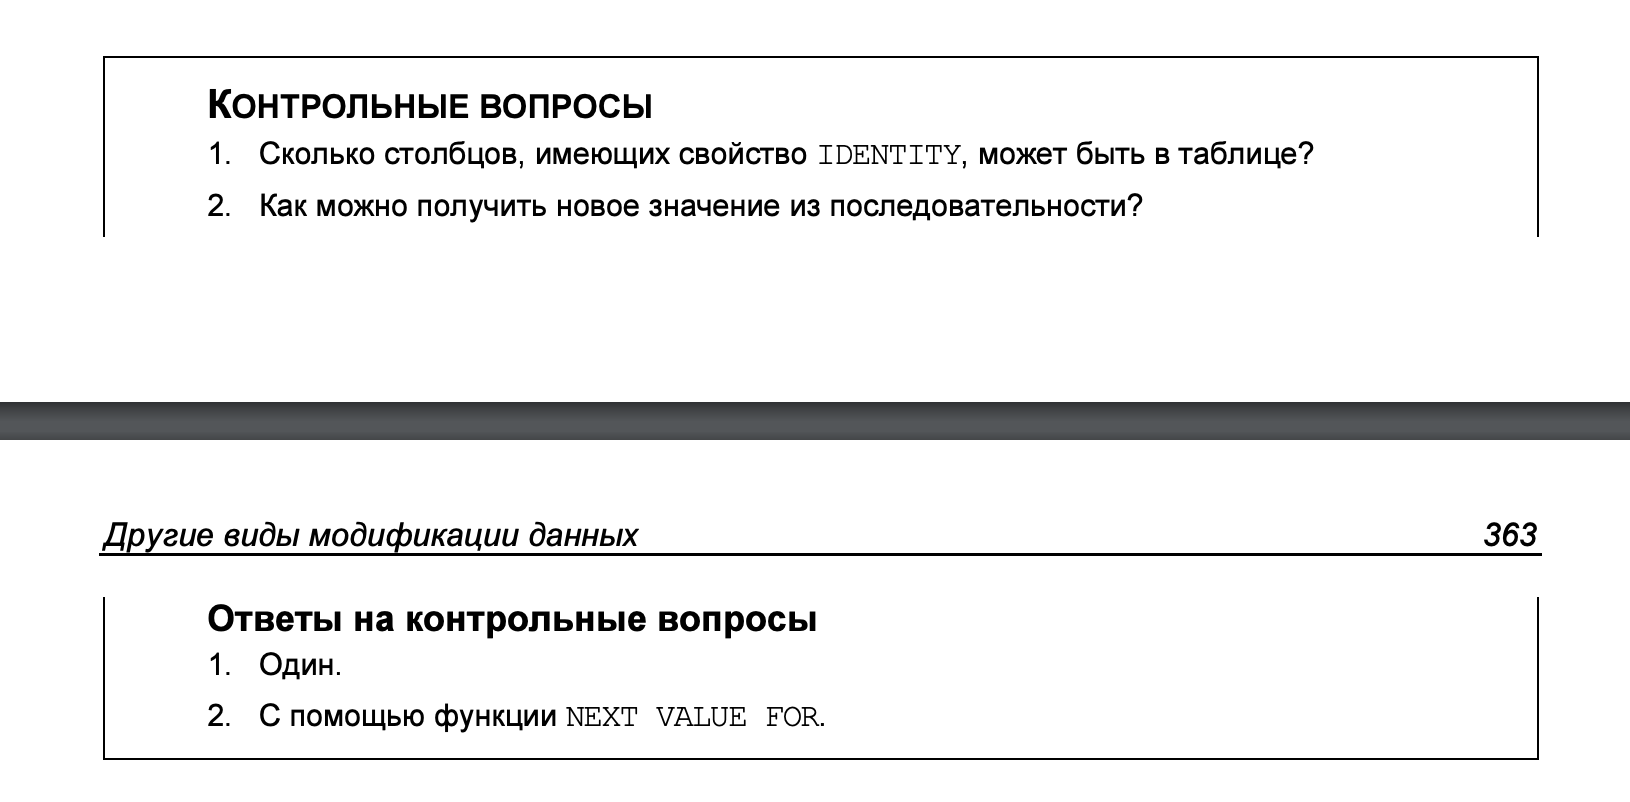
\includegraphics[width=0.6\textwidth]{img/control24.png}
	\end{center}
	\captionsetup{justification=centering}
\end{figure}


\subsection*{Резюме занятия}
\begin{itemize}
	\item SQL Server поддерживает две возможности, позволяющие генерировать последовательность ключей: свойство столбца IDENTITY и объект последовательности. 
	\item Свойство столбца IDENTITY определяется с начальным значением и приращением. При вставке новой строки в целевую таблицу вам не нужно указывать
	значение для столбца IDENTITY, вместо этого SQL Server генерирует его автоматически.
	\item Чтобы получить вновь сгенерированное свойство идентификатора, можно выполнить запрос с помощью функций COPE\_IDENTITY, @@IDENTITY и IDENT\_CURRENT.
	Первая возвращает последнее значение идентификатора, сгенерированное
	в данном сеансе и диапазоне. Вторая возвращает последний идентификатор,
	сгенерированный в данном сеансе. Третья возвращает последний идентификатор, сгенерированный во входной таблице. 
	\item Объект последовательности — это независимый объект в базе данных. Он не
	привязан к определенному столбцу в конкретной таблице. 
	\item Объект последовательности поддерживает определение начального значения,
	значения приращения, минимального и максимального поддерживаемых значений, циклического повторения и кэширования. 
	\item Функция NEXT VALUE FOR используется для запроса нового значения из последовательности. Эту функцию можно применять в инструкциях INSERT и UPDATE,
	ограничениях DEFAULT и присвоениях значений переменным. 
	\item Объект последовательности обходит многие ограничения свойства IDENTITY. 
\end{itemize}

\subsection*{Закрепление материала}

\begin{figure}[h!]
	\begin{center}
		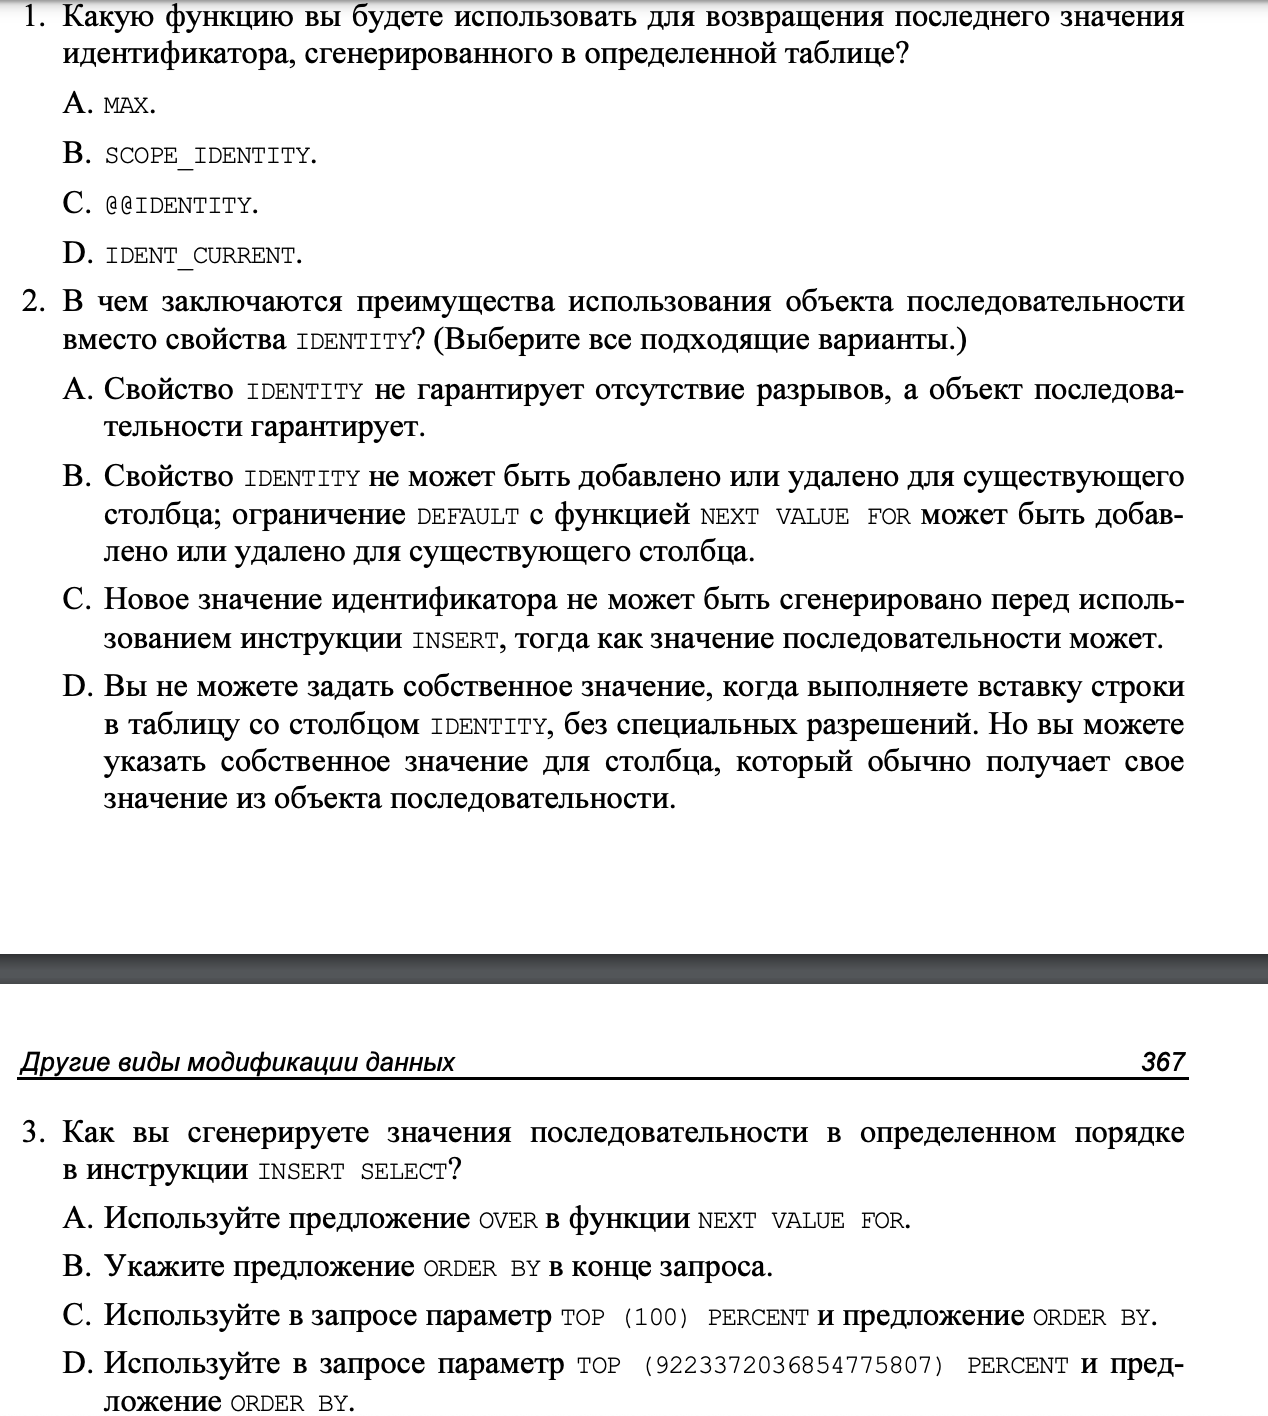
\includegraphics[width=0.9\textwidth]{img/zakrep25.png}
	\end{center}
	\captionsetup{justification=centering}
\end{figure}
\newpage

\subsection*{Ответы}

\begin{figure}[h!]
	\begin{center}
		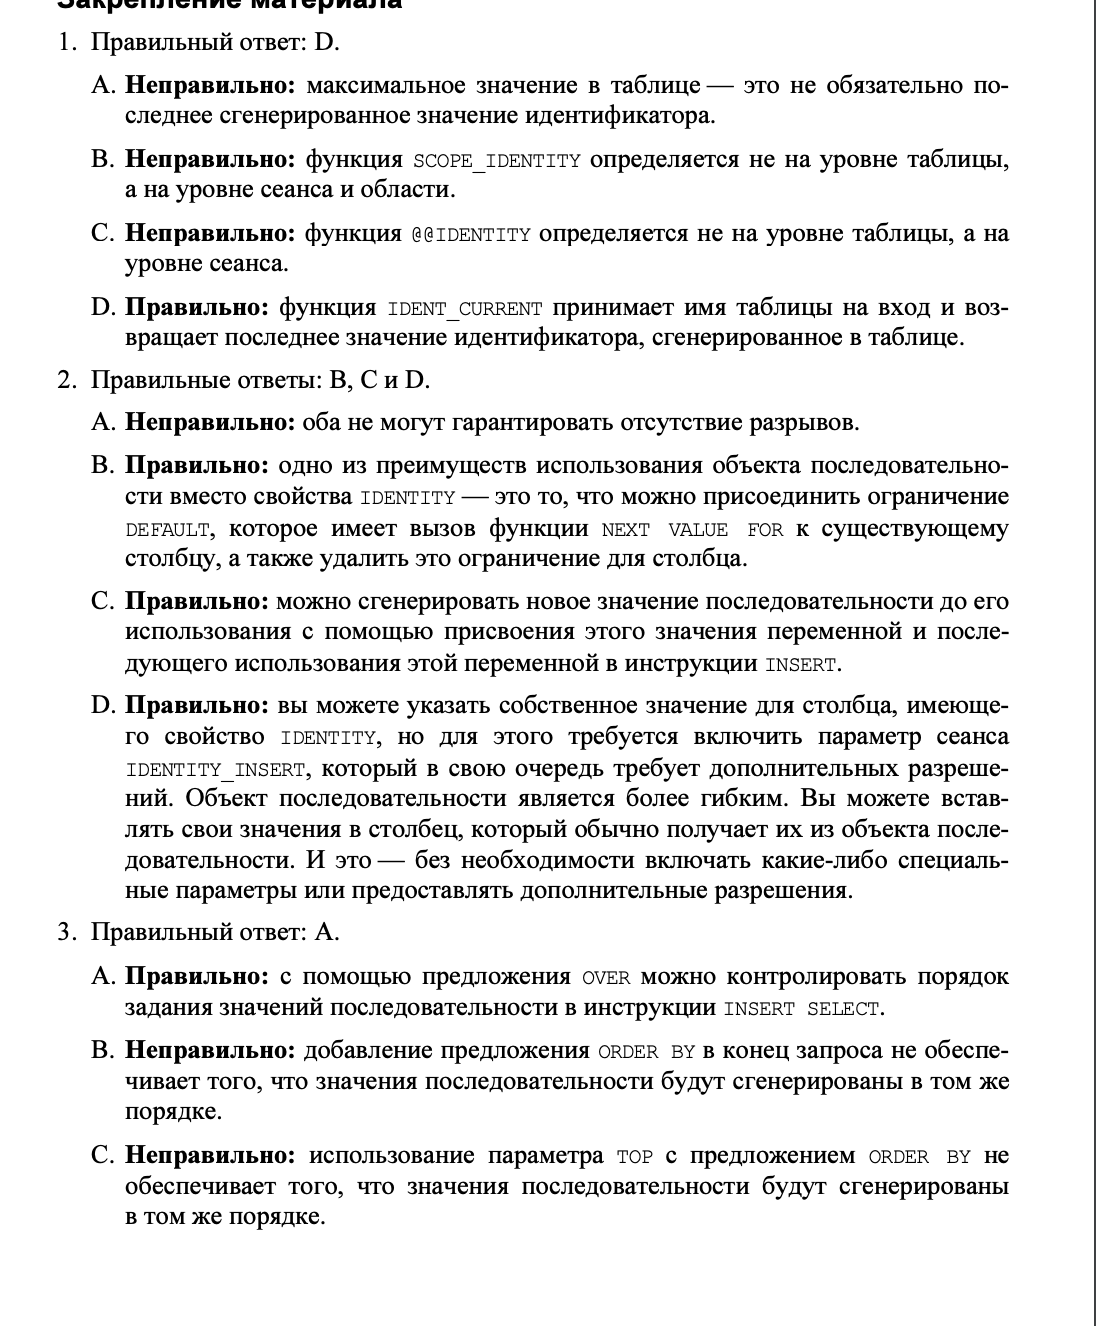
\includegraphics[width=0.9\textwidth]{img/ans25.png}
	\end{center}
	\captionsetup{justification=centering}
\end{figure}
\clearpage


\section{Слияние данных}

\subsection{Использование инструкции MERGE}

С помощью инструкции MERGE выполняется слияние данных из исходной таблицы
или табличного выражения и целевой таблицы с помещением их в целевую таблицу. Общий формат инструкции MERGE выглядит следующим образом: 

\begin{lstlisting}[label=lst:funcReturn, language=sql]
	MERGE INTO <target table> AS TGT
	USING <SOURCE TABLE> AS SRC
	ON <merge predicate>
   WHEN MATCHED [AND <predicate>] 
	THEN <action> 
   WHEN NOT MATCHED [BY TARGET] [AND <predicate>] 
	
	THEN INSERT...
   WHEN NOT MATCHED BY SOURCE [AND <predicate>] 
	THEN <action>; 
\end{lstlisting}

Далее перечислены предложения этой инструкции и их роли. 

\begin{itemize}
	\item MERGE INTO <target table>. Это предложение определяет целевую таблицу
	(target table) данной операции. При желании можно задать псевдоним таблицы
	в этой операции. 
	\item USING <source table>. Это предложение определяет исходную таблицу (source
	table) для данной операции
	\item ON <merge predicate>. В этом предложении вы указываете предикат (merge
	predicate), который выполняет сопоставление строк между источником и целевой таблицей и определяет, имеется или нет целевая строка, соответствующая
	исходной строке. Обратите внимание, это предложение не является фильтром,
	как, например, предложение ON в соединении. 
	\item WHEN MATCHED [AND <predicate>] THEN <action>. Это предложение определяет
	действие (action), которое следует предпринять, если строке источника соответствует целевая строка. 
	\item 
\end{itemize}

\begin{figure}[h!]
	\begin{center}
		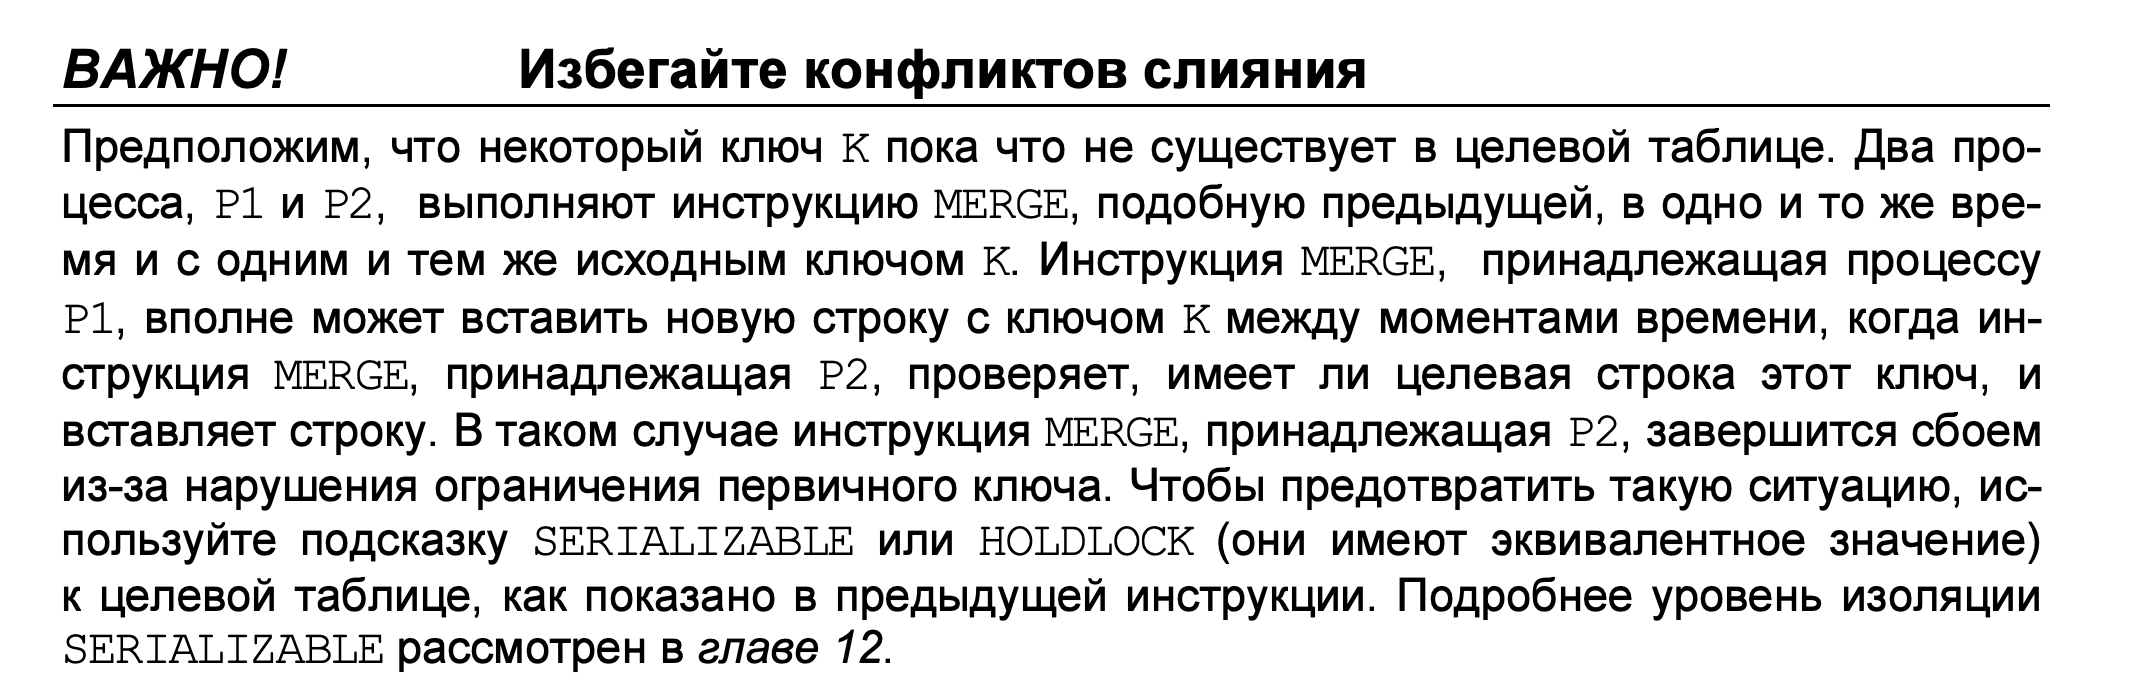
\includegraphics[width=0.9\textwidth]{img/advice22.png}
	\end{center}
	\captionsetup{justification=centering}
\end{figure}

\begin{figure}[h!]
	\begin{center}
		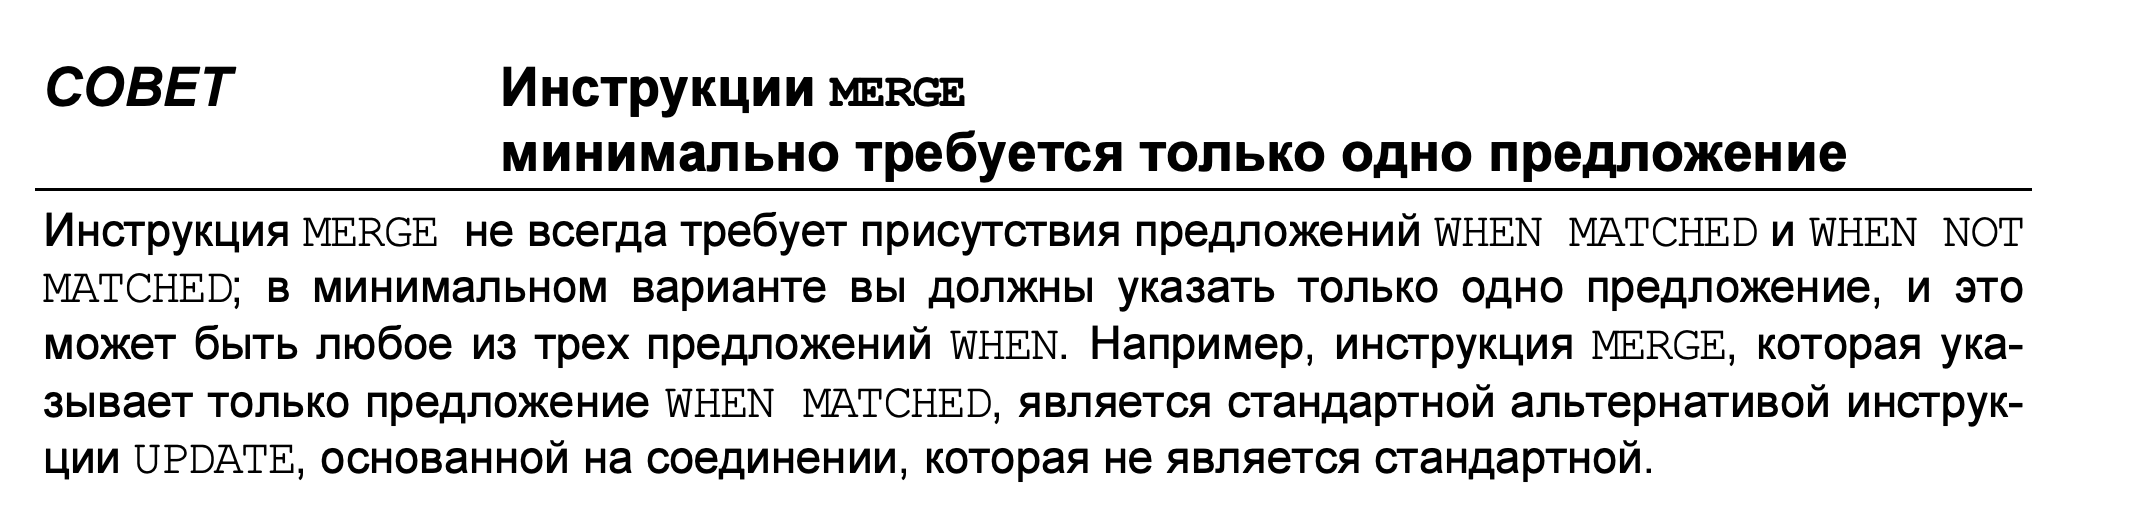
\includegraphics[width=0.9\textwidth]{img/advice23.png}
	\end{center}
	\captionsetup{justification=centering}
\end{figure}


\begin{figure}[h!]
	\begin{center}
		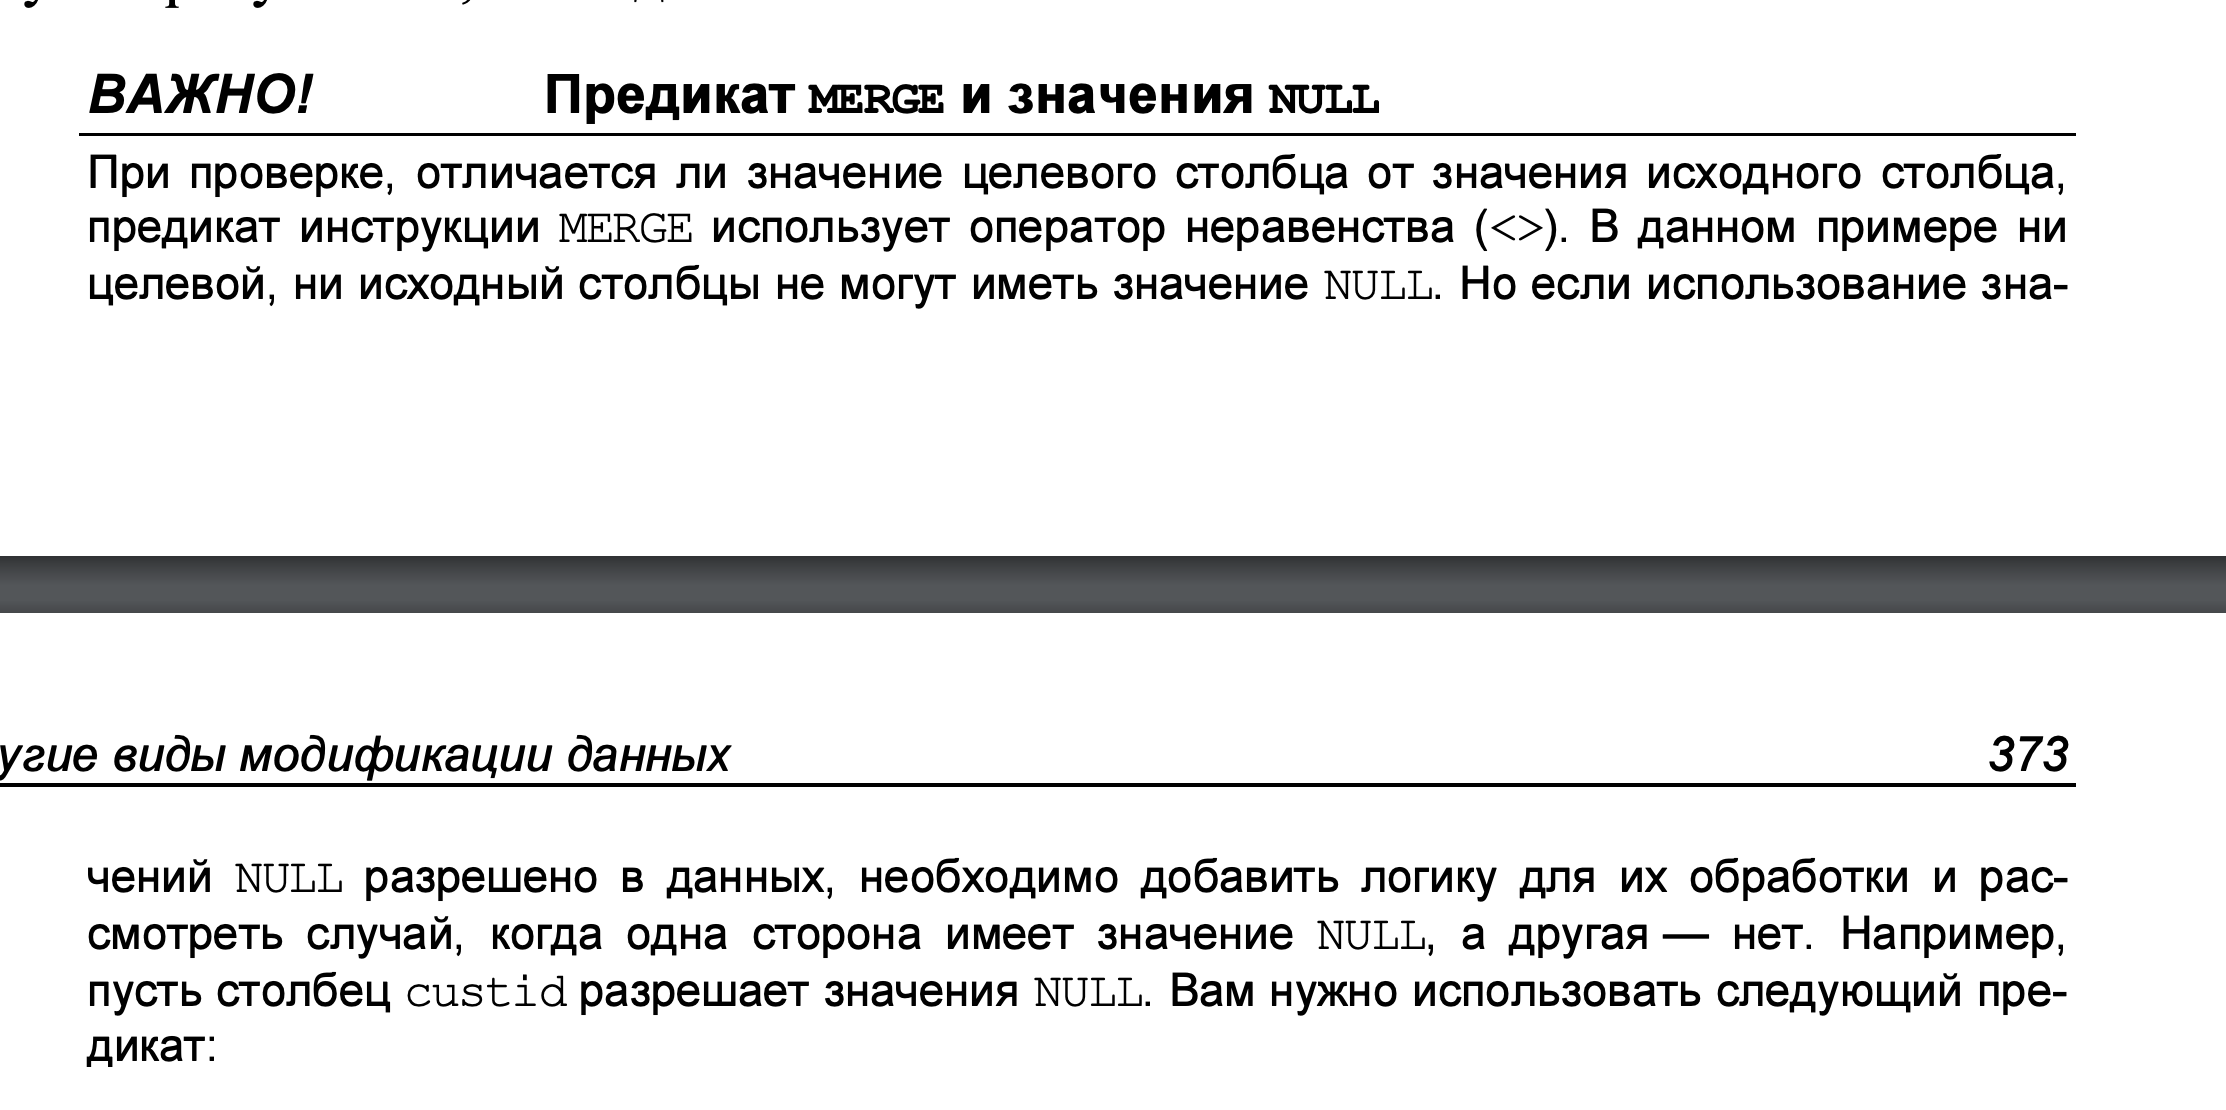
\includegraphics[width=0.9\textwidth]{img/control25.png}
	\end{center}
	\captionsetup{justification=centering}
\end{figure}
		
\subsection*{Резюме занятия}
\begin{itemize}
	\item С помощью инструкции MERGE можно выполнить слияние данных из исходной
	таблицы или табличного выражения в целевую таблицу. 
	\item Целевую таблицу указывают в предложении MERGE INTO, а исходную таблицу —
	в предложении USING. Предложение USING похоже на предложение FROM инструкции SELECT, что означает возможность использования табличных операторов,
	табличных выражений, табличных функций и пр. 
	\item Предикат слияния указывается в предложении ON, которое определяет, сопоставляется ли строке источника целевая строка и сопоставляется ли целевой строке
	строка источника. Помните, что предложение ON не используется для фильтрации данных; напротив, оно служит только для определения соответствия или несоответствия строк и для определения действий, которые следует применить
	к целевой таблице.
	\item Должны быть определены разные предложения WHEN, которые указывают, какое
	действие применить к целевой таблице в зависимости от выходных данных предиката. Можно указать действия, которые следует выполнить, когда исходной
	строке соответствует целевая строка, когда исходной строке не соответствует ни
	одна целевая строка и когда целевой строке не соответствует исходная строка. 
\end{itemize}

\subsection*{Закрепление материала}

\begin{figure}[h!]
	\begin{center}
		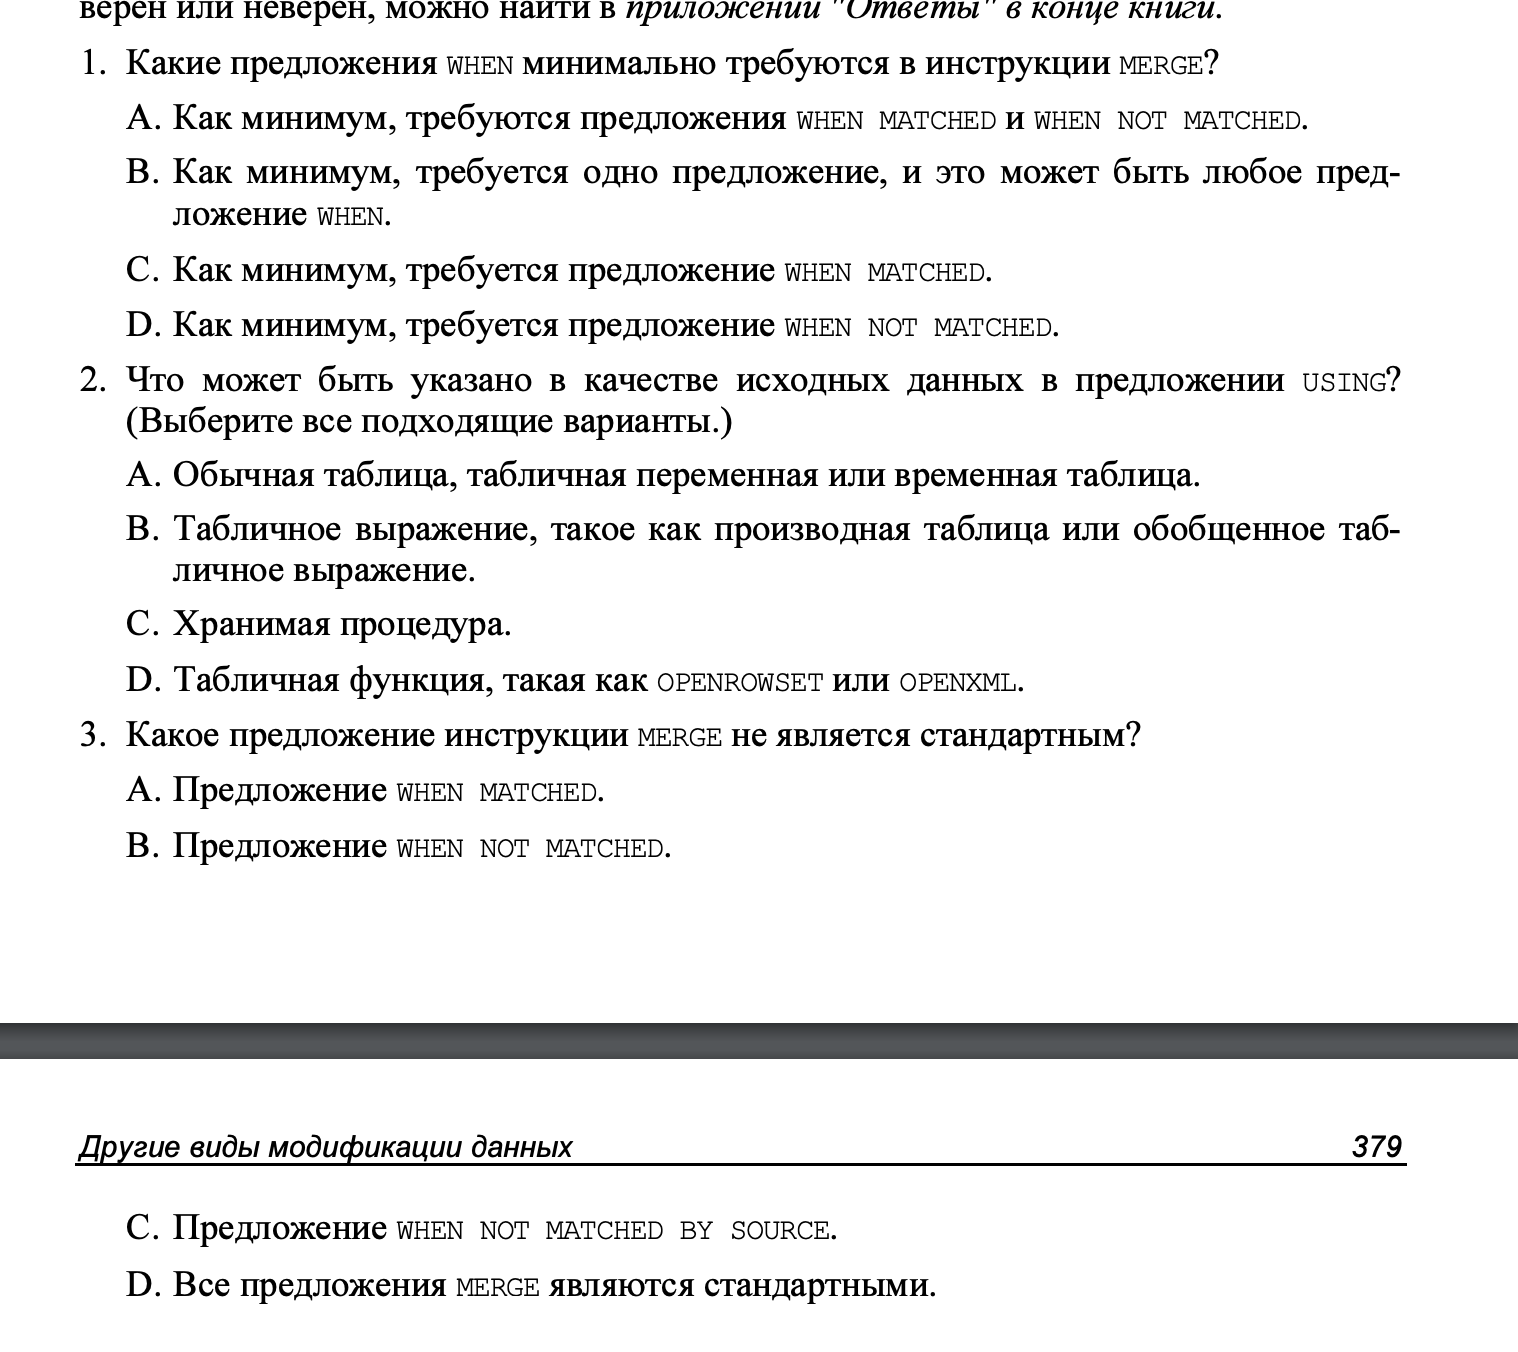
\includegraphics[width=0.9\textwidth]{img/zakrep22.png}
	\end{center}
	\captionsetup{justification=centering}
\end{figure}
\clearpage

\subsection*{Ответы}

\begin{figure}[h!]
	\begin{center}
		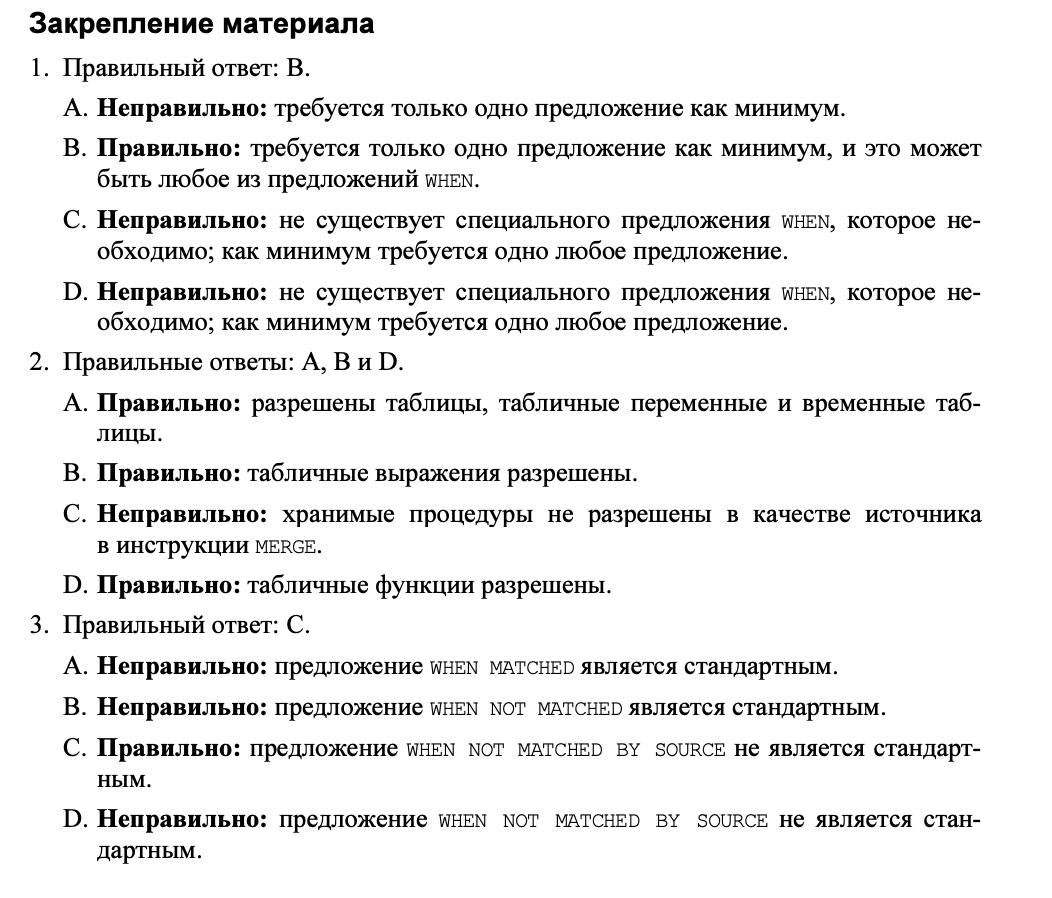
\includegraphics[width=0.9\textwidth]{img/ans24.png}
	\end{center}
	\captionsetup{justification=centering}
\end{figure}


\section{Использование предложения OUTPUT}

\subsection{Инструкция INSERT с предложением OUTPUT}

Предложение OUTPUT может использоваться в инструкции INSERT для того, чтобы
возвращать информацию из вставленных строк. Примером его практического использования может служить многострочная инструкция INSERT, которая генерирует
новые ключи с помощью свойства IDENTITY или последовательности, а вам нужно
знать, какие новые ключи были сгенерированы. 


\begin{lstlisting}[label=lst:funcReturn, language=sql]
	INSERT INTO Sales.MyOrders(custid, empid, orderdate)
	OUTPUT
	inserted.orderid, inserted.custid, inserted.empid, inserted.orderdate
	SELECT custid, empid, orderdate
	FROM Sales.Orders
	WHERE shipcountry = N'Norway';
\end{lstlisting}

Если вам нужно сохранить результат в таблице, а не возвращать его назад вызывающей стороне, добавьте предложение INTO с именем целевой таблицы следующим образом: 

\begin{lstlisting}[label=lst:funcReturn, language=sql]
	INSERT INTO Sales.MyOrders(custid, empid, orderdate)
	OUTPUT
	inserted.orderid, inserted.custid, inserted.empid, inserted.orderdate
	INTO SomeTable(orderid, custid, empid, orderdate)
	SELECT custid, empid, orderdate
	FROM Sales.Orders
	WHERE shipcountry = N'Norway'; 
\end{lstlisting}

\subsection{Инструкция DELETE с предложением OUTPUT}

\begin{lstlisting}[label=lst:funcReturn, language=sql]
	DELETE FROM Sales.MyOrders
	OUTPUT deleted.orderid
   WHERE empid = 1; 
\end{lstlisting}

\subsection{Инструкция UPDATE с предложением OUTPUT}

\begin{lstlisting}[label=lst:funcReturn, language=sql]
	UPDATE Sales.MyOrders
	SET orderdate = DATEADD(day, 1, orderdate)
	OUTPUT inserted.orderid,
	deleted.orderdate AS old_orderdate,
	inserted.orderdate AS neworderdate
   WHERE empid = 7; 
\end{lstlisting}

\subsection{Инструкция MERGE с предложением OUTPUT}

SQL Server предоставляет функцию action. Эта функция возвращает строку
('INSERT', 'UPDATE' или 'DELETE'), обозначающую выполненную операцию. 

\begin{lstlisting}[label=lst:funcReturn, language=sql]
MERGE INTO Sales.MyOrders AS TGT
USING (VALUES(1, 70, 1, '20061218')
 (2, 70, 7, '20070429')
AS SRC(orderid, custid, empid, orderdate)
 ON SRC.orderid = TGT.orderid
WHEN MATCHED AND (TGT.custid <> SRC.custid
 OR TGT.empid <> SRC.empid
 OR TGT.orderdate <> SRC.orderdate) THEN UPDATE
SET TGT.custid = SRC.custid,
 TGT.empid = SRC.empid,
 TGT.orderdate = SRC.orderdate
WHEN NOT MATCHED THEN INSERT
 VALUES(SRC.orderid, SRC.custid, SRC.empid, SRC.orderdate)
WHEN NOT MATCHED BY SOURCE THEN
 DELETE
OUTPUT
 $action AS the_action,
 COALESCE(inserted.orderid, deleted.orderid) AS orderid; 
\end{lstlisting}

\begin{figure}[h!]
	\begin{center}
		
\includegraphics[width=0.9\textwidth]{img/advice24.png}
	\end{center}
	\captionsetup{justification=centering}
\end{figure}


\subsection{Компонуемый DML }

В качестве примера компонуемого DML рассмотрим предыдущую инструкцию MERGE . Предположим, что вам нужно получить лишь строки, к которым
применялась только операция INSERT, и передать их в табличную переменную для последующей обработки. Этого можно достигнуть с помощью следующего
кода: 

\begin{lstlisting}[label=lst:funcReturn, language=sql]
SELECT orderid, custid, empid, orderdate
FROM (MERGE INTO Sales.MyOrders AS TGT 
	...
	...
	...
	...
	OUTPUT
 		$action AS the_action, inserted.*) AS D
WHERE the_action = 'INSERT';
\end{lstlisting}

\begin{figure}[h!]
	\begin{center}
		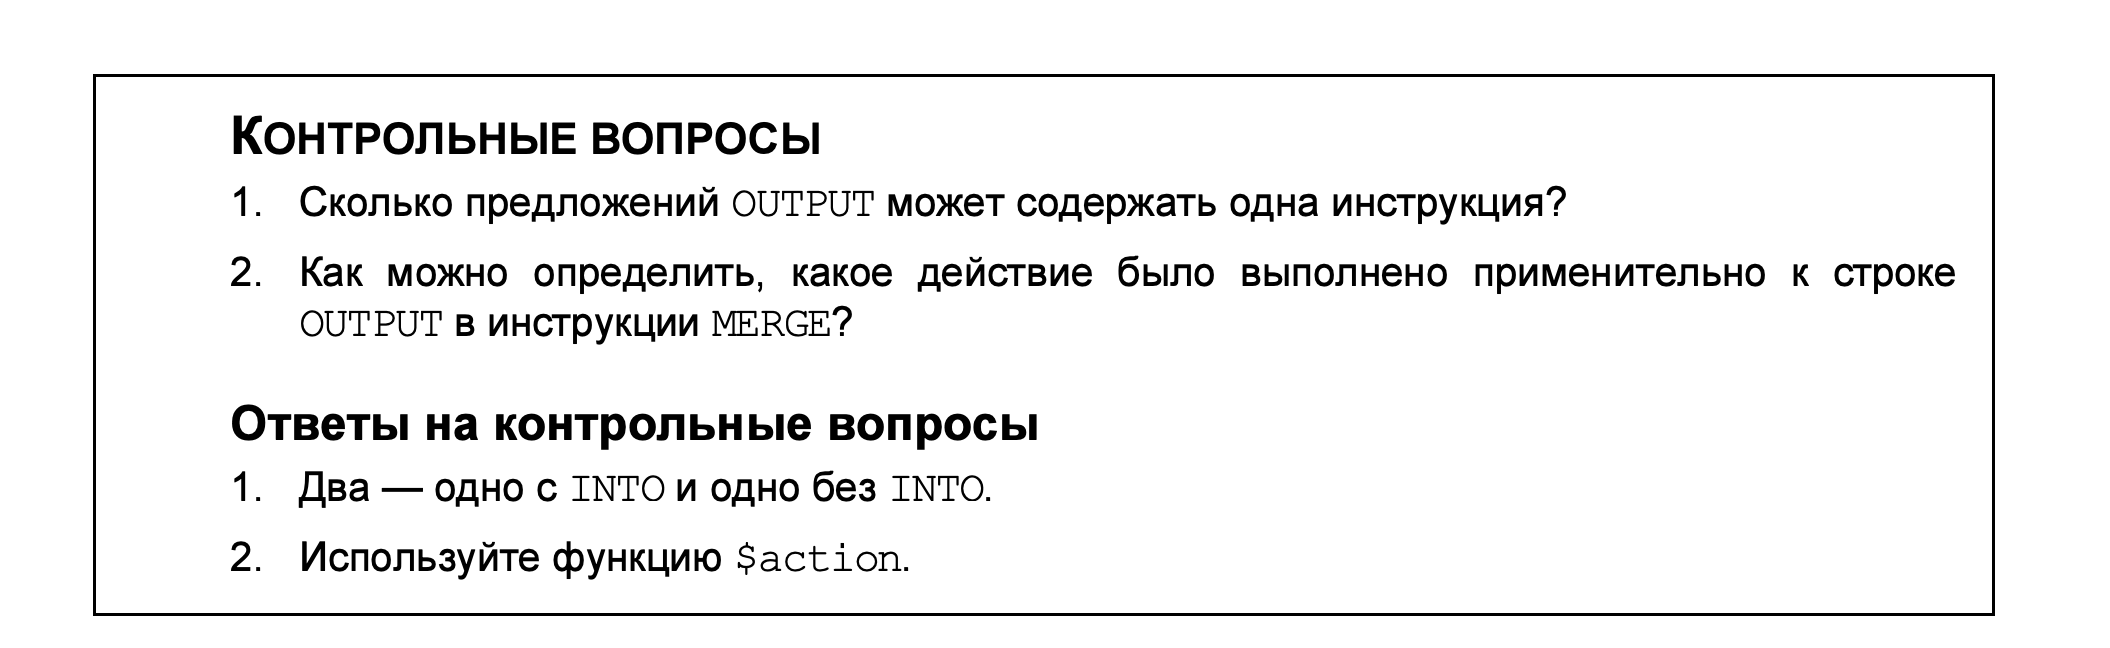
\includegraphics[width=0.9\textwidth]{img/control27.png}
	\end{center}
	\captionsetup{justification=centering}
\end{figure}


\subsection*{Резюме занятия}
\begin{itemize}
	\item С помощью предложения OUTPUT можно возвращать информацию из измененных
	строк в инструкциях модификации. 
	\item Предложение OUTPUT построено как предложение SELECT, что позволяет формировать выражения и присваивать результирующим столбцам псевдонимы. 
	\item Результат предложения OUTPUT можно отправить обратно вызывающей стороне
	в виде результирующего набора из запроса или сохранить в целевой таблице
	с помощью предложения INTO. 
	\item При ссылке на столбцы из модифицированных строк следует присваивать в качестве префикса именам столбцов ключевое слово inserted для вставленных
	строк и deleted для удаленных строк. 
	\item В инструкции MERGE можно использовать функцию action для возвращения
	строки, которая представляет действие, примененное к целевой строке. 
	\item Компонуемый DML следует использовать для фильтрации выходных строк, которые необходимо сохранить в целевой таблице. 
\end{itemize}


\subsection*{Закрепление материала}

\begin{figure}[h!]
	\begin{center}
		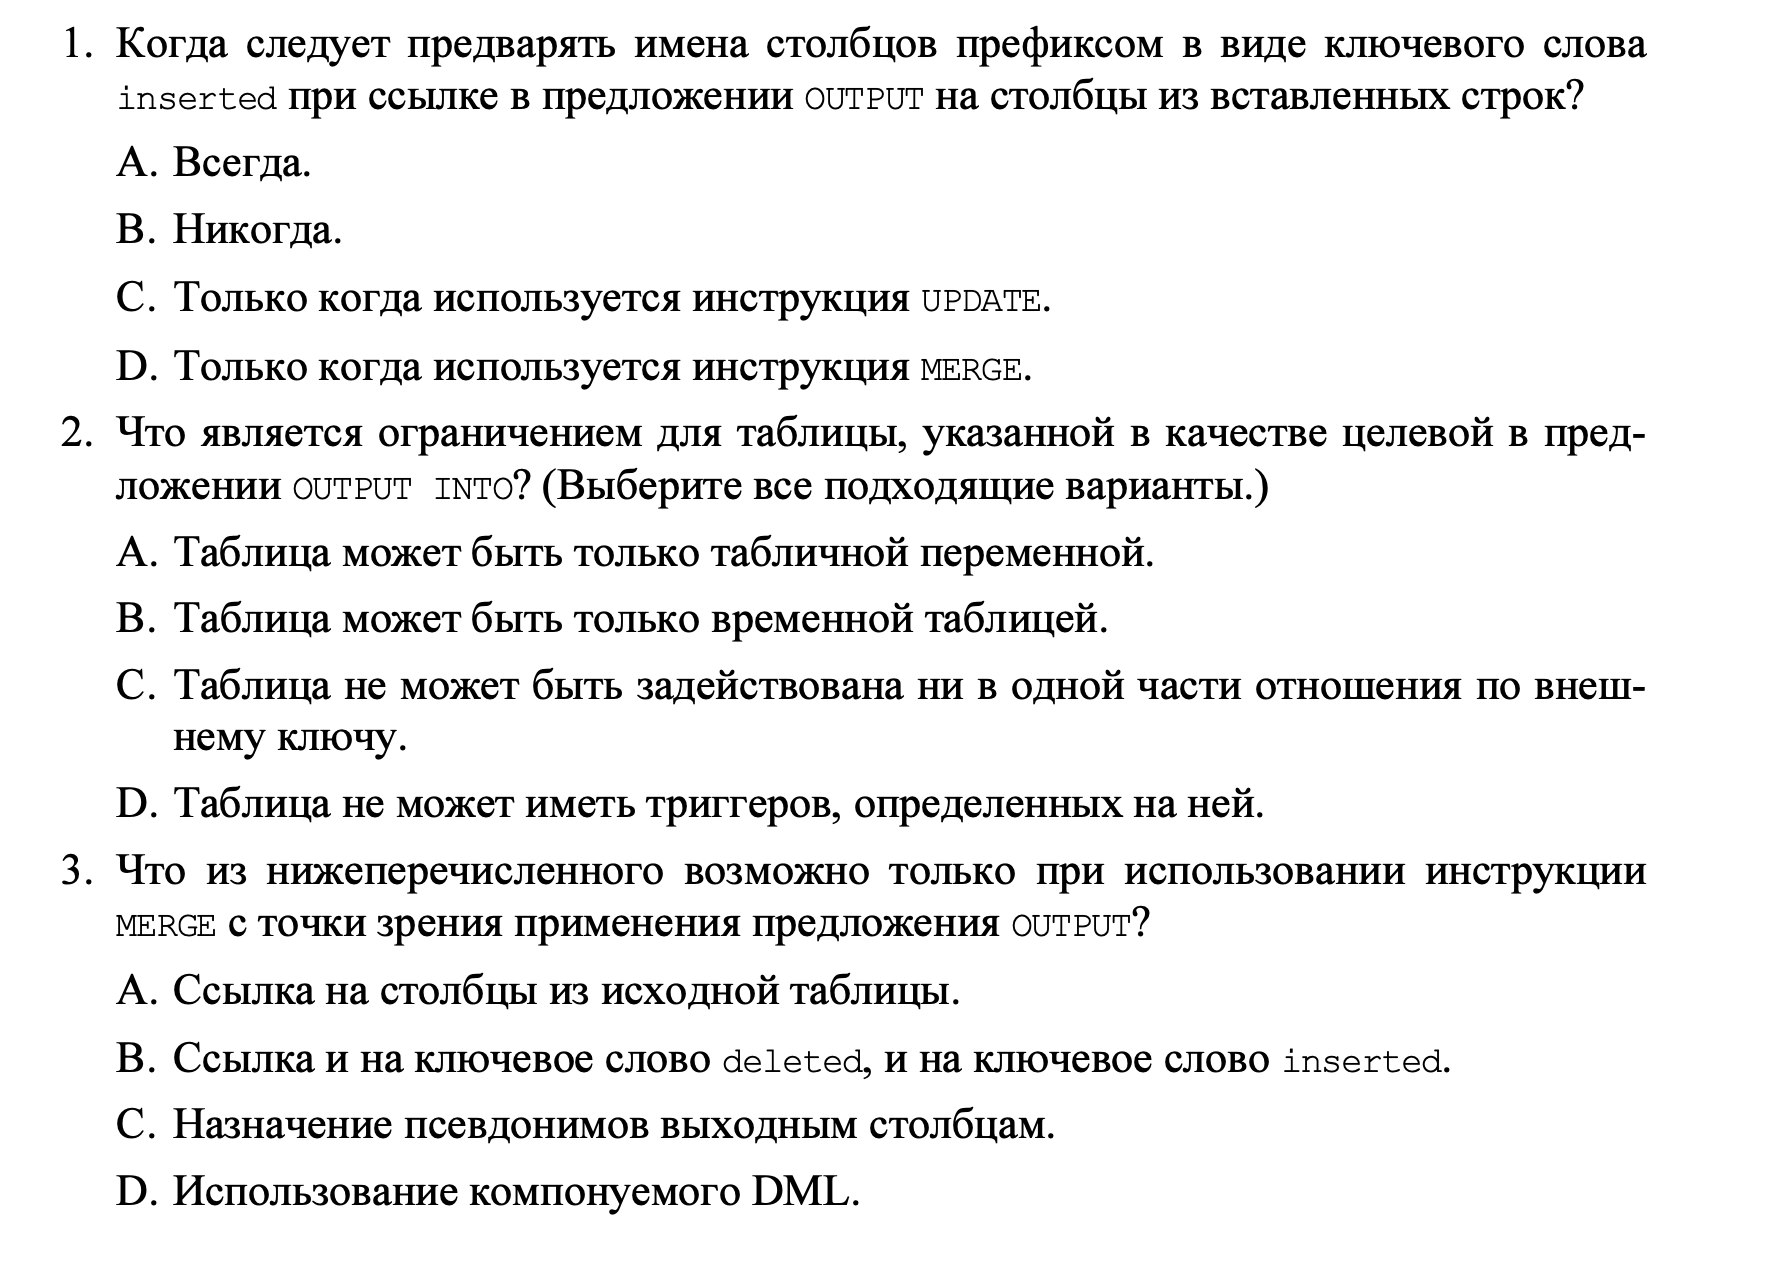
\includegraphics[width=0.7\textwidth]{img/zakrep26.png}
	\end{center}
	\captionsetup{justification=centering}
\end{figure}
\clearpage

\subsection*{Ответы}

\begin{figure}[h!]
	\begin{center}
		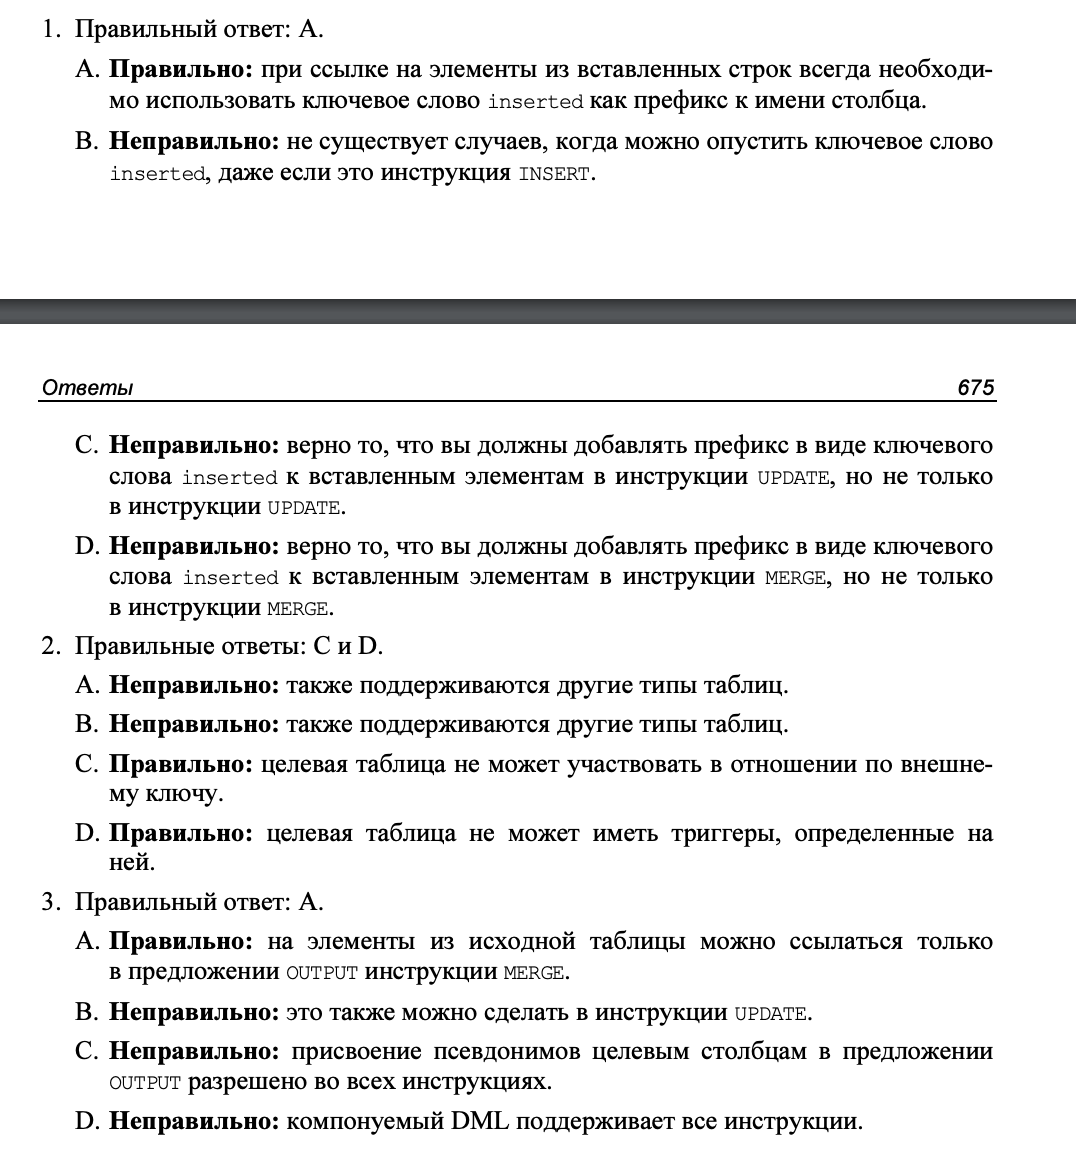
\includegraphics[width=0.9\textwidth]{img/ans26.png}
	\end{center}
	\captionsetup{justification=centering}
\end{figure}


\newpage
\subsection*{Упражнения}

\begin{figure}[h!]
	\begin{center}
		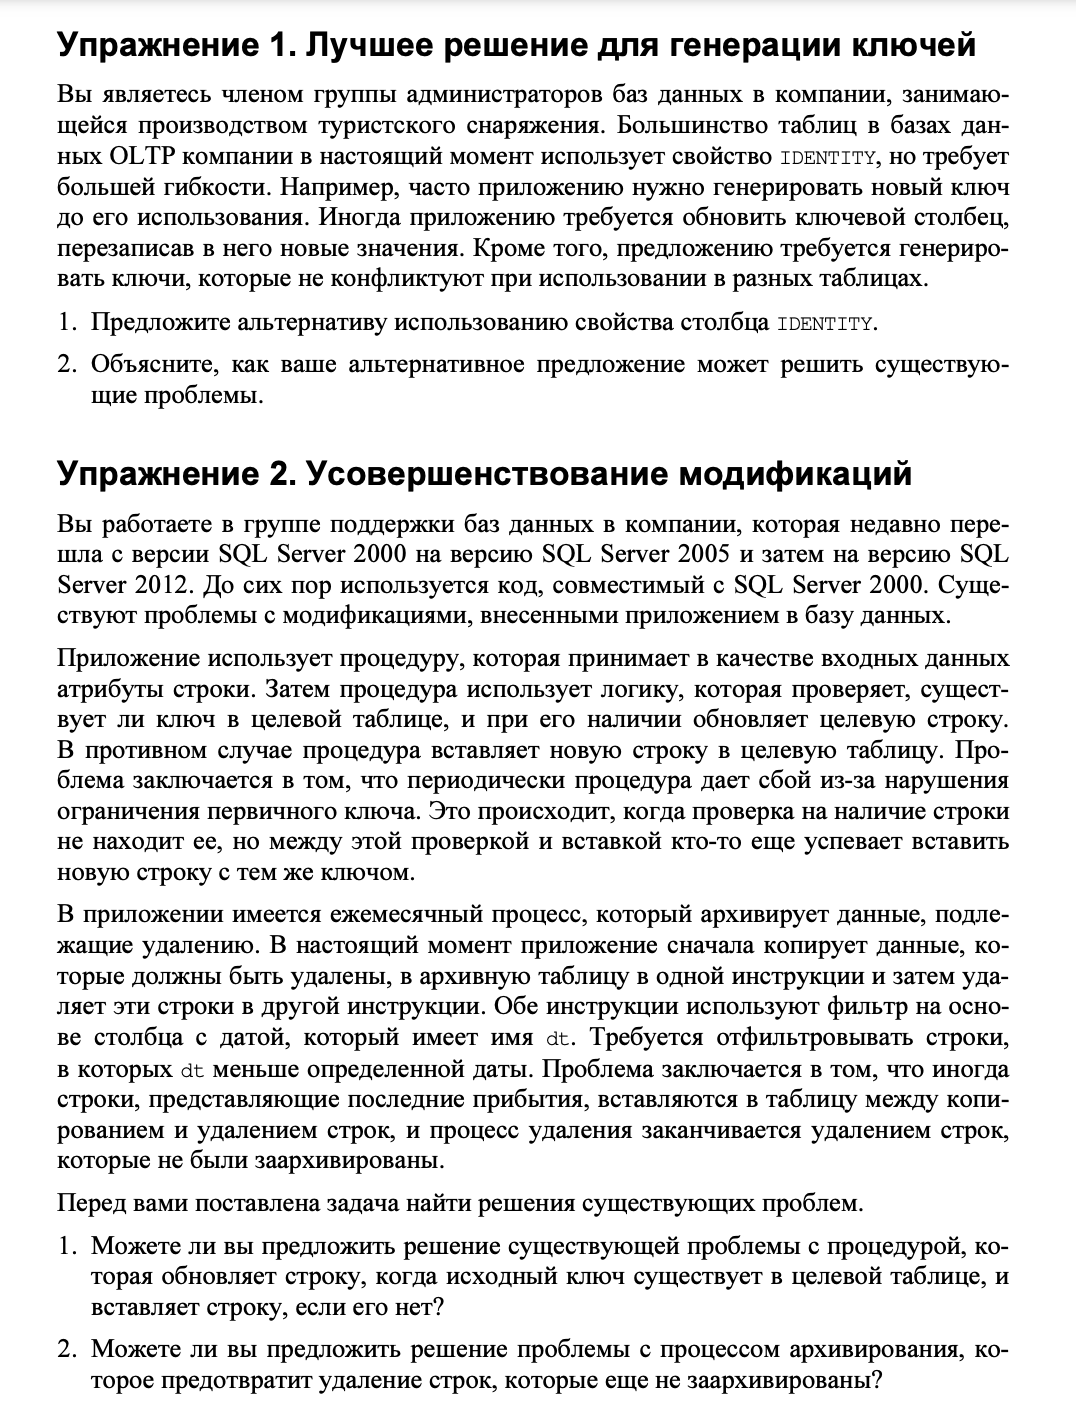
\includegraphics[width=0.9\textwidth]{img/ex17.png}
	\end{center}
	\captionsetup{justification=centering}
\end{figure}

\subsection*{Ответы}

\begin{figure}[h!]
	\begin{center}
		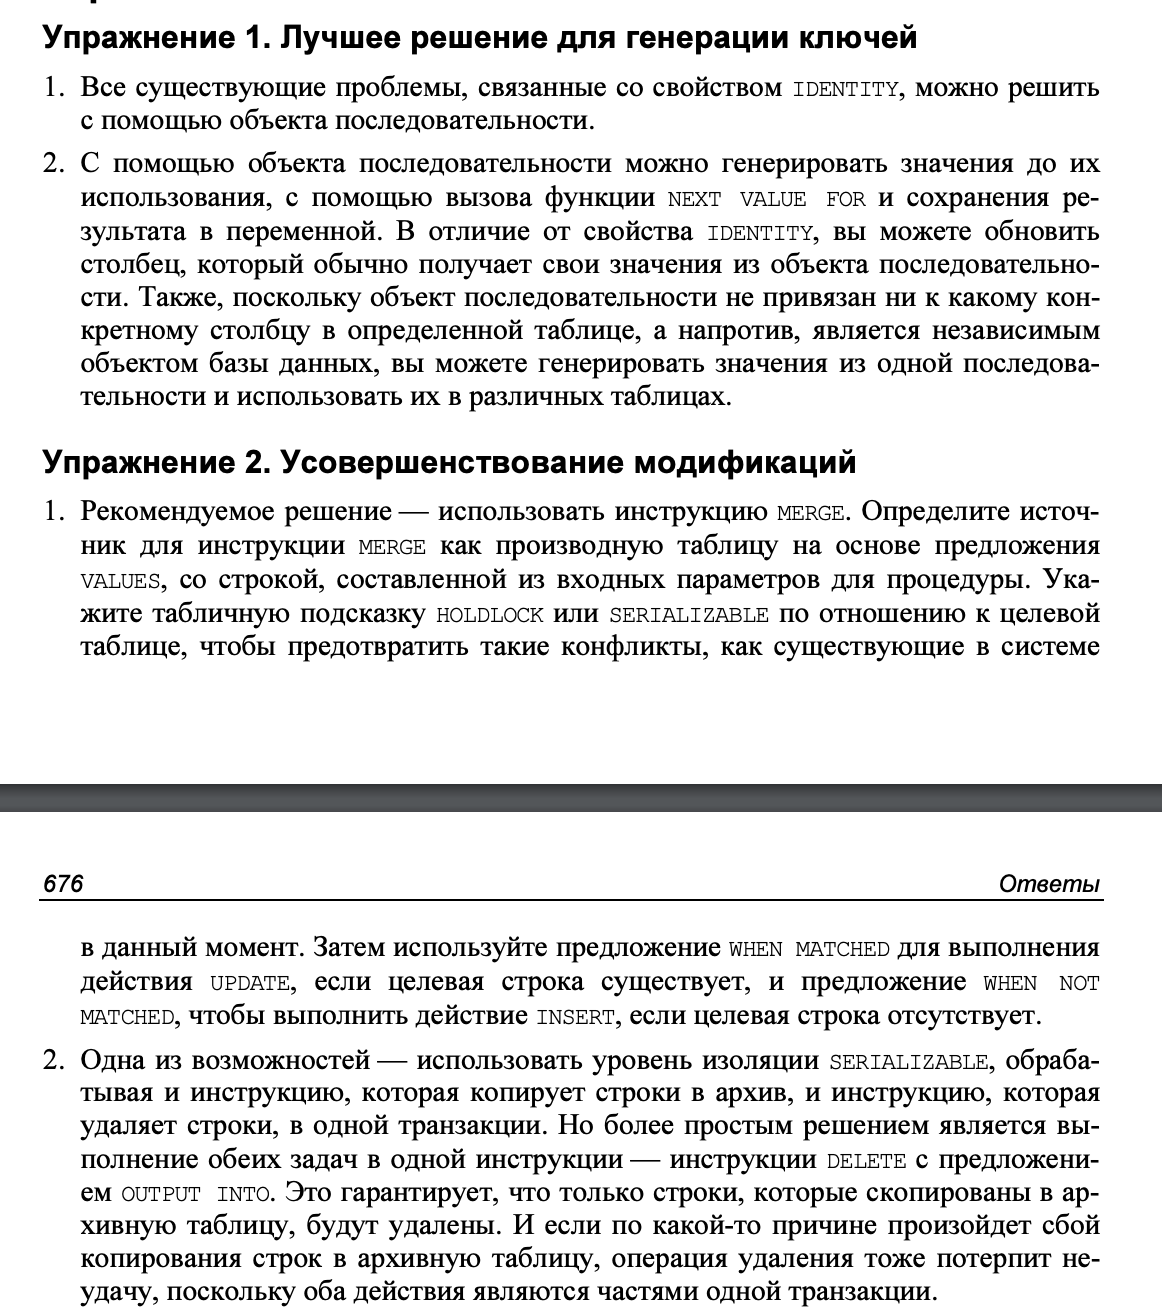
\includegraphics[width=0.9\textwidth]{img/eans17.png}
	\end{center}
	\captionsetup{justification=centering}
\end{figure}





